% vim: set tw=78 sts=2 sw=2 ts=8 aw et ai:

The architecture of the \textit{Hive} simulator can be seen in Figure 1.

\begin{figure}[htb]
  \begin{center}
    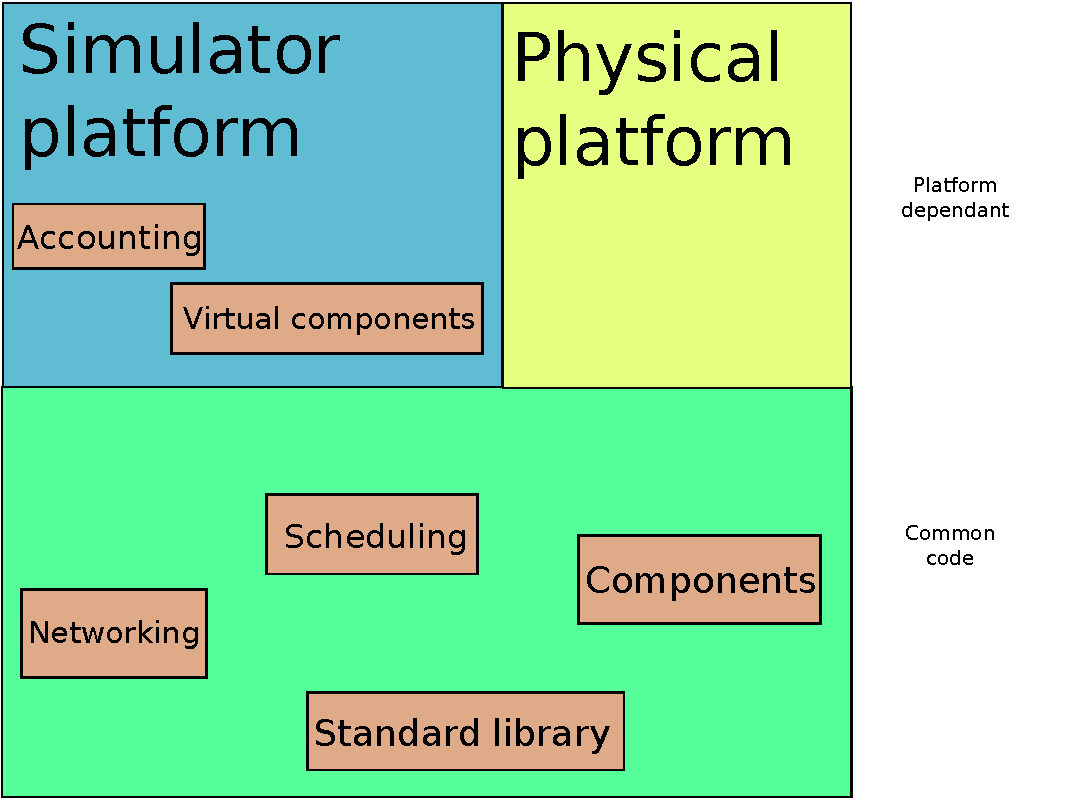
\includegraphics[scale=0.75]{img/bigarch.pdf}
    \caption{Hive Simulator Architecture}
  \end{center}
\end{figure}

The \textit{Hive} simulator can be broken into three parts:
\begin{itemize}
  \item Plugin or node specific code
  \item Platform agnostic code accessed by a standard library
  \item Platform specific code used by the standard library
\end{itemize}

A wireles sensor node running in a \textit{Hive} simulation is 
represented by a dynamic library, which we will call plugin. This library contains the code 
which would normally run on the node, with a few simple extra methods
so it can be used in the simulator. This library will be loaded once
for each node type.

The plugin will set timers to schedule work on the node. Let's say that we have
a node with two sensors, a temperature sensor and a noise sensor. Upon
initialisation, the sensor will set a timer to run once every 5 minutes to
read temperature and another one for the noise sensor to run once every
minute. The plugin will collect the data from these sensors in the internal memory
and set a timer to send the data to a master node once every 30 minutes.
Apart from scheduling work to be done, the plugin can also interact with other
node by sending data. It uses an API similar to BSD sockets that abstract the
networking system.

The simulator is implemented as a platform for \textit{Hive}. It has its own scheduler
and implementation for network devices. Code running on the simulated node
will always pass through the scheduler so the simulator can take appropriate
actions based on the event.

\subsection{Networking}

The \textit{Hive} simulator has support for the 6LowPAN and ZigBee stack protocols.

\subsubsection{6LowPAN\cite{6lowpan}}
A LoWPAN is a simple low cost communication network that allows
wireless connectivity in applications with limited power and relaxed
throughput requirements. A LoWPAN typically includes devices that
work together to connect the physical environment to real-world
applications, e.g., wireless sensors. LoWPANs conform to the IEEE
802.15.4-2003 standard.


\subsubsection{ZigBee}
ZigBee is a technology used in automation and remote control applications that
provides low data rate, low power, low consumption wireless networking. It is mainly
used in equipments that require long battery life but not high transfer rate as those
enabled by Bluetooth.
ZigBee uses the functionality and standardisation of the physical layer and
medium access control layer defined in IEEE 802.15.4 for LoWPANs to which it then adds
a couple of layers: the network layer, and the application layer and two main
components: the ZigBee device objects (ZDOs) and manufacturer-defined application objects.
The last two components allow customization of applications which could define
their own behaviours and, also, total integration.


\subsection{Controlling the simulator}

The simulator is controlled through simple commands on a TCP socket. For
example to load a test plugin, start it, stop it and then unload it we would
do:
\begin{lstlisting}
$ nc 127.0.0.1 54321
load test
1
start 1
stop 1
unload 1
\end{lstlisting}

If the library test.so is not found in LD\_LIBRARY\_PATH an error will be
thrown.
